
% \documentclass[14pt]{extarticle}
\documentclass[bibliography=totocnumbered]{scrartcl}
% \usepackage[english]{babel}
\usepackage[russian]{babel}
\usepackage[utf8x]{inputenc}
\usepackage{amsmath}
\usepackage{graphicx}
\usepackage[colorinlistoftodos]{todonotes}
\usepackage{amssymb}
\usepackage{amsmath}
\usepackage{graphicx}
\usepackage[margin=.8in]{geometry}
\usepackage{listings}
\usepackage[section]{placeins}
\usepackage{listings}
\begin{document}


\begin{titlepage}
\newgeometry{margin=2cm}
\newcommand{\HRule}{\rule{\linewidth}{0.5mm}} % Defines a new command for the horizontal lines, change thickness here

\center % Center everything on the page
 
%----------------------------------------------------------------------------------------
%	HEADING SECTIONS
%----------------------------------------------------------------------------------------
\textsc {
\footnotesize{
минобрнауки россии\\
федеральное государственное бюджетное образовательное учреждение\\
высшего профессионального образования}\\
\large{Воронежский государственный университет}
}\\[1.0cm] % Name of your university/college


\textsc{\largeФакультет компьютерных наук}\\ % Major heading such as course name
\textsc{\footnotesizeКафедра информационных технологий}\\[1.0cm] 
\textsc{\Large Отчет по научно-исследовательской работе}\\[0.5cm] % Minor heading such as course title


%----------------------------------------------------------------------------------------
%	TITLE SECTION
%----------------------------------------------------------------------------------------

\HRule \\[0.4cm]
{ \huge \bfseries Возможности построения реальных сенсорных сетей}\\[0.4cm] % Title of your document
\HRule \\[1.5cm]
 
%----------------------------------------------------------------------------------------
%	AUTHOR SECTION
%----------------------------------------------------------------------------------------


\begin{flushleft} \large
\emph{Зав. кафедрой:} Ю.Б. \textsc{Нечаев}, д. ф-м н., проф.\\
\emph{Студент:} А.А. \textsc{Валиков}, 1 курс маг. \\ % Your name
\emph{Руководитель:} А.В. \textsc{Стромов} % Supervisor's Name
\end{flushleft}

\begin{center}
Воронеж 2018
\end{center}
\end{titlepage}

\tableofcontents

\newpage 

\section{Введение}
Всё большее распространение получают системы умного дома. Перед инженерами встаёт всё больше технических препятствий на пути реализации подобных систем, например такие как автономность устройств, процессом сбора данных с большого числа датчиков, обработка собранной информации и принятие требуемых решений. \\
Для больших распределённых систем с большим количеством обрабатываемой информации препочтительным способом реализации сети сенсоров может являться беспроводная сенсорная сеть. \\ 
При этом могут рассматриваться как случаи мобильных датчиков (так называемые MANET) и стационарные сети.

\section{Цель}

Исследование характеристик реальных сенсорных сетей. Конкретнее, ведётся работа по следующим направлениям:

\begin{itemize}

\item Увеличение время жизни сети (снижение энергопотребления). Доведение в идеале одного сенсорного юнита до такого энергопотребления, чтобы имелась возможность использовать автомоные источники питания при нечастой подзарядке.

\item Оценить численно, какое количество информации может «снять» сеть из окружающего мира без потерь данных. Также проварьировать число участников сети. Разработать алгоритмы, позволяющие максимально приблизиться к теоретическому пределу таких сетей.

\end{itemize}

\section{Теоретическое обоснование}

\subsection{Топология}
Важнейшей характеристикой сети является её \textbf{топология} . Для сетей как правило используются:
\begin{itemize}
	\item Звезда
	\item Кластерное дерево
	\item Меш
\end{itemize}

В этой работе предполагается использование топологии меш, где каждый узел связан с несколькими своими соседями, и в сети присутствет один узел сбора информации.

\begin{figure}[htp]
\centering
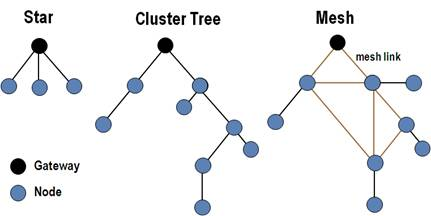
\includegraphics[scale=1.00]{topology.jpg}
\end{figure}

\subsection{Компоненты сенсорного узла}

Необходимыми компонентами сенсорного узла являются:
\begin{itemize}
	\item Микроконтроллер
	\item Сенсорные датчики
	\item Источник питания (как правило батарея)
	\item Радиопередатчик
\end{itemize}

\begin{figure}[htp]
\centering
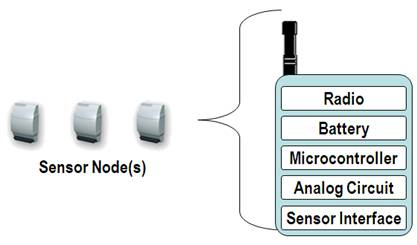
\includegraphics[scale=1.00]{components.jpg}
\end{figure}



\section{Описание возможностей модуля, используемого в работе}

\begin{itemize}

\item HC-11 - беспроводной модуль, работающий на частоте 434 МГц.

\item Пользователю не нужно программировать модуль, только четыре режима отвечают за прием и отправку данных последовательного порта.

\item Низкое потребление тока: 80 мкА, 3.5 мA, 22 мA, в зависимости от выбранного режима.

\item Неограниченное число байтов, передаваемое одновременно (но часть может быть потеряна)


\item Все параметры сохраняются в памяти даже в случае отключения питания.


\item Рабочее напряжение: 3.3 - 5В

\end{itemize}

\subsection{Режимы функционирования}

\begin{itemize}

\item \textbf{FU1 Стандартный режим }
   
Потребление тока: $3.4mA$.

\item \textbf{FU2 Максимальное энергосбережение}

Задержка сигнала: $400ms$
  
Скорость передачи (симв.): $1200, 2400, 4800$
 
Потребление тока: $80\mu A$

\item \textbf{FU3 Максимальная скорость}

Задержка сигнала: $< 10 ms$ 

Потребление тока: $23 mA$.

\item \textbf{FU4 Максимальное расстояние}

Задержка сигнала: $>300ms$ 

Скорость передачи (симв.): $9,600$ 

Потребление тока: $22mA$.

\end{itemize}


\subsection{Команды}


В скобках указаны переменные


\begin{enumerate}

\item \textbf{AT}

Тестовая команда. Если всё нормально, модуль возвращает OK.

\begin{tabular}{ l r }
  Отправляем: & AT \\
  Получаем: & OK \\
\end{tabular}


\item \textbf{ AT+A(000-255)}

Меняет адрес модуля в указанном диапазоне.

\begin{tabular}{ l l }
  Отправляем: & AT+A012 \\
  Получаем: & OK-A012 \\
\end{tabular}


\item \textbf{ AT+B(1200 | 2400 | 4800 | 9600 | 19200 | 38400 | 57600 | 115200)}

Меняет скорость (baud rate) на одно из допустимых значений (указаны выше).

\begin{tabular}{ l l }
  Отправляем: & AT+B19200 \\
  Получаем: & OK-B19200 \\
\end{tabular}


\item \textbf{ AT+C(001-127)}

Меняет канал беспроводного соединения. Нули перед числами обязательны. Если значение слишком большое, данные могут быть потеряны. Так что, на самом деле доступны каналы $001-020$.


\begin{tabular}{ l l }
  Отправляем: & AT+C015 \\
  Получаем: & OK-C015 \\
\end{tabular}


\item \textbf{AT+E(A | B | C)(соответствующие числа)}

Эта команда используется для управления удалённым модулем.

\begin{itemize}
\item Первый параметр - три выше описанные команды (адрес (A), скорость (B) и канал (C) соответственно)
\item Второй - значение, которое мы хотим присвоить выбранному параметру
\end{itemize} 


Возвращаемые значения:

\begin{tabular}{ l l }
  Успех: & \\
  E(A | B | C)R & успех \\
\end{tabular}

\begin{tabular}{ l l }
  Ошибки: & \\
  E(A | B | C)E & ошибка параметра \\
  E(A | B | C)F & ошибка команды \\
  Fail & ошибка соединения \\
\end{tabular}

\textbf{Пример 1}

Устанавливаем адрес удалённого модуля в $050$

\begin{tabular}{ l l }
  Отправляем: & AT+EA050 \\
  Получаем: & OK-EBR \\
\end{tabular}

\textbf{Пример 2}

Устанавливаем скорость удалённого модуля в $4800$

\begin{tabular}{ l l }
  Отправляем: & AT+EB4800 \\
  Получаем: & OK-EBR \\
\end{tabular}

\item \textbf{ AT+FC(M | S)(F | T) }

Устанавливает модуль в режим IO управления.

Первый параметр:
\begin{itemize}
\item M - управляюший
\item S - управляемый 
\end{itemize}

Второй
\begin{itemize}
\item F - повторяющий
\item T - обратный
\end{itemize}

\begin{tabular}{ l l }
  Один модуль отправляет: & AT+FCMT, чтобы стать управляющим \\
  Другой отправляет: & AT+FCST, чтобы стать управляемым \\
\end{tabular}


\item \textbf{AT+FU(1-4)}

Переключает в один из режимов, описанных выше.

\begin{tabular}{ l l }
  Отправляем: & AT+FU1 \\
  Получаем: & OK-FU1 \\
\end{tabular}


\item \textbf{AT+GDPCxAx}

Устаревшая команда.
  
\item \textbf{AT+P(1-8)}

Устанавливает мощность передатчика

\begin{tabular}{ l l }
  Отправляем: & AT+P6 \\
  Получаем: & OK-P6 \\
\end{tabular}

  
\item \textbf{AT+R(A | B | C | P)}

Получает значение одного из параметров

\begin{tabular}{ l l }
  Отправляем: & AT+RB \\
  Получаем: & B9600 \\
\end{tabular}

\begin{tabular}{ l l }
  Отправляем: & AT+RA \\
  Получаем: & A001 \\
\end{tabular}


\item \textbf{AT+U(N | O | E)(1 | 2 | 3)}

Устанавливает бит проверки данных и бит завершения последовательного порта.

Первый параметр:

\begin{itemize}
\item N - нет проверки
\item O - нечётный
\item E - чётный 

\end{itemize}

Второй параметр:
\begin{itemize}
\item 1 - стоп-бит
\item 2 - 2 бита
\item 3 - 1.5 бита

\end{itemize}

\begin{tabular}{ l l }
  Отправляем: & AT+UO2 \\
  Получаем: & UO2 \\
\end{tabular}

  
\item \textbf{AT+RX}

Получает значения всех параметров модуля:  
режим последовательного порта / скорость / канал / адрес / мощность 

\begin{tabular}{ l l }
  Отправляем: & AT+RX \\
  Получаем: & U1 B9600 C001 A000 P8 \\
\end{tabular}

\item \textbf{AT+V}

Получает версию прошивки.

\begin{tabular}{ l l }
  Отправляем: & AT+V \\
  Получаем: & HC-11\_V1.3\\
\end{tabular}



\item \textbf{AT+SLEEP}

Переводит модуль в спящий режим после выхода из AT. В этом режиме не возможна передача данных. Чтобы выйти из спящего режима, нужно войти в AT ещё раз. Эта команда доступна с версии $1.8$.

Потребление тока: $20 \mu A$.

\begin{tabular}{ l l }
  Отправляем: & AT+SLEEP \\
  Получаем: & OK\\
\end{tabular}



\item \textbf{AT+RESET}

Сбрасывает последовательный порт, канал и адрес в стандартные значения.

\begin{tabular}{ l l }
  Отправляем: & AT+RESET \\
  Получаем: & RESET\_OK\\
\end{tabular}


\item \textbf{AT+IV}

Получает версию внутреннего кода управления. Команда доступна с версии $1.9$

\begin{tabular}{ l l }
  Отправляем: & AT+IV \\
  Получаем: & I1\\
\end{tabular}


\item \textbf{AT+UPDATE}

Переводит модуль в режим ожидания обновления.
После отправки команды модуль не будет отвечать на команды до перезагрузки.
После того как контроллер последовательного порта отправит команду, закройте последовательный порт, выберите файл в помощнике обновления HC-11, откройте последовательный порт. Затем модуль сможет обновиться

\end{enumerate}

\subsection{Рекомендации по использованию модуля}

Если расстояние между модулями слишком маленькое (меньше 50 см), стоит установить мощность передачи небольшой (P1 - P3). Иначе, передача будет перенасыщена и соединение не удастся. Если расстояние составляет несколько сантиметров, передача, вероятно, не получится.

\section{Описание программы}

\subsection{Прошивка для arduino}
Программа представляет собой код, ожидающий поступления команд с серийного порта, и дейсвующий по двум сценариям:
\begin{itemize}
	\item Команды \lstinline{config.enable} и \lstinline{config.disable} соответственно включают и отключат режим конфигурирования для модуля arduino.
	\item Любая другая команда отправляется напрямую в модуль. Команды для модуля имую синтакис \lstinline{AT+...}, где ... один из допустимых параметров модуля.
\end{itemize} 
Код программы
\begin{lstlisting}

#include <SoftwareSerial.h>
SoftwareSerial radio(3, 4);
int setPin = 2;

String command = "";


void setup() {

  Serial.begin(9600);
  radio.begin(9600);

  pinMode(setPin, OUTPUT);
  digitalWrite(setPin, HIGH);

  getConfigStatus();
}



void loop() {

  command = readSerial();

  if (command.length() > 0) {
    if (command == "config.enable") {
      enableConfig();
    }

    else if (command == "config.disable") {
      disableConfig();
    }

    else if (command == "config.status") {
      getConfigStatus();
    }

    else {
      radio.print(command);
      Serial.println("MESSAGE: " + command);
    }
  }

  readRadio();

  delay(500);

  command = "";
}

void enableConfig() {
  digitalWrite(setPin, LOW);
  Serial.println("Config enabled");
}

void disableConfig() {
  digitalWrite(setPin, HIGH);
  Serial.println("Config disabled");
}

void getConfigStatus() {
  if (digitalRead(setPin) == 0) {
    Serial.println("CONFIG=TRUE");
  } else {
    Serial.println("CONFIG=FALSE");
  }
}



String readSerial() {
  String command = "";

  while (Serial.available() > 0) {
    command += char(Serial.read());
  }

  return command;
}

String readRadio() {
  String response = "";

  while (radio.available() > 0) {
    response += char(radio.read());
  }

  if (response.length() > 0) {
    response = "RESPONSE: " + response;
    Serial.print(response);
    return response;
  }

}
\end{lstlisting} 

\subsection{Бек-энд на Java Spring}
Бэк-энд является прослойкой между фронт-эндом, где планируется размещение основной логики и собственно Arduino с модулем. Код, описывающий контроллер, обрабатывающий запросы к веб-серверу.

\begin{lstlisting}
package somepackage;
import arduino.*;
import somepackage.Flower;
import somepackage.FlowerRepository;
import javax.annotation.PostConstruct;

@Controller
@RequestMapping(path="/arduino_radio")
public class FlowerController {

  private Arduino arduino;

  @PostConstruct
  void afterInit() {
    arduino = new Arduino("ttyUSB1", 9600);
    arduino.openConnection();
  }

  @GetMapping(path="/disable_config")
  public @ResponseBody void disableConfig() {
    arduino.serialWrite("config.disable");
  }
}
\end{lstlisting}

\subsection{Фронт-энд на Angular}
Фронт-энд предполагает наличие UX элементов для управления параметрами модуля, такими как канал, дальность и другие. На данный момент фронт-энд находится в разработке, также возможно в будущем изменится цель проекта, что приведёт к переписыванию модуля.

\section{Вывод}
Большое количество настроек (адрес, канал, скорость) и четыре режима позволяют предположить широкие вохможности модуля HC-11 для создания сенсорных сетей:
 
\begin{itemize}
\item Распределённых на большое расстояние (режим FU4)
\item Имеющих большое кол-во участников на единицу площади (20 каналов и 255 адресов)
\item Требующих высокой скорости передачи (режим FU3)

\item Сильно ограниченных по запасу энергии (режим FU2 и спящий режим)

\end{itemize}


\section{Заключение}
\newpage

\begin{thebibliography}{9}
\bibitem{latexcompanion} 
National Instruments / What Is a Wireless Sensor Network?
\\\texttt{http://www.ni.com/white-paper/7142/en/}
 

\bibitem{knuthwebsite} 
Wireless sensor network
\\\texttt{https://en.wikipedia.org/wiki/Wireless\char`_sensor\char`_network}

\bibitem{suisse} 
Internet of Things: Wireless Sensor Networks
\\\texttt{http://www.iec.ch/whitepaper/pdf/iecWP-internetofthings-LR-en.pdf}

\bibitem{radio} 
HC-11 Wireless Serial Port Module
\\\texttt{https://www.elecrow.com/download/HC-11.pdf}

\end{thebibliography}


\end{document}